%%%%%%%%%%%%%%%%%%%%%%%%%%%%%%  IEEEsample.tex
%%%%%%%%%%%%%%%%%%%%%%%%%%%%%%%%%%%%%%%%%
%%%%%%%%%%%%%%%%%%%%%%%    More information: see the header of IEEEtran.sty
%%%%%%%%%%%%%%%%%%%%%%%
%%%%%%%%%%%%%%%%%%%%%%%%%%%%%%%%%%%%%%%%%%%%%%%%%%%%%%%%%%%%%%%%%%%%%%%%%%%%%%%%
%%%%

\documentclass[conference,10pt]{IEEEtran}
%\documentclass[conference]{IEEEtran}

%%%\IEEEoverridecommandlockouts

%\usepackage[ruled]{./algorithm2e}
%%for algorithm2e package, label has to be following caption in the same line!!!
%\renewcommand{\algorithmcfname}{ALGORITHM}
%\SetAlFnt{\small}
%\SetAlCapFnt{\small}
%\SetAlCapNameFnt{\small}
%\SetAlCapHSkip{0pt}
%\IncMargin{-\parindent}



%% \RequirePackage{times}
%% \RequirePackage{algorithmic}
%% \PassOptionsToPackage{boxed}{algorithm}
%% \RequirePackage{algorithm}
%% \RequirePackage{multicol}
%\renewcommand{\algorithmicrequire}{\textbf{Inputs:}}
%\renewcommand{\algorithmicensure}{\textbf{Outputs:}}
%\DeclareMathAlphabet{\mathtsl}{OT1}{ptm}{m}{sl}

%\def\BibTeX{{\rm B\kern-.05em{\sc i\kern-.025em b}\kern-.08em1
%    T\kern-.1667em\lower.7ex\hbox{E}\kern-.125emX}}

%\newtheorem{theorem}{Theorem}
%\newtheorem{lemma}{Lemma}
%\newtheorem{example}{Example}
%\newtheorem{corollary}{Corollary}

\RequirePackage{amssymb, mathptm}
\usepackage{amsbsy}
\usepackage{graphicx}
\usepackage{helvet}
\usepackage{enumerate}
\usepackage{amsmath}
\usepackage{amsfonts}
\usepackage{graphicx}
\usepackage{multirow}
\usepackage{subfig}
\usepackage{comment}
\usepackage{leqno}
\usepackage{cases}
\usepackage{multirow}


\usepackage{algorithm}
\usepackage{algorithmicx}
\usepackage{algpseudocode}
\usepackage{graphicx}
\usepackage{listings}
\lstset{language=C}



%%indent in algorithm


%\setcounter{page}{1}


% New command for the table notes.
\def\tabnote#1{{\small{#1}}}

% New command for the line spacing.
\newcommand{\ls}[1]
    {\dimen0=\fontdimen6\the\font
     \lineskip=#1\dimen0
     \advance\lineskip.5\fontdimen5\the\font
     \advance\lineskip-\dimen0
     \lineskiplimit=.9\lineskip
     \baselineskip=\lineskip
     \advance\baselineskip\dimen0
     \normallineskip\lineskip
     \normallineskiplimit\lineskiplimit
     \normalbaselineskip\baselineskip
     \ignorespaces
    }
%\renewcommand{\algorithmicrequire}{\textbf{Input:}}
%\renewcommand{\algorithmicensure}{\textbf{Output:}}

\newcommand{\beq}{\begin{equation}}
\newcommand{\eeq}{\end{equation}}
\newcommand{\beqarr}{\begin{eqnarray}}
\newcommand{\eeqarr}{\end{eqnarray}}
%\newcommand{\ov}{\overline}
\newcommand{\ov}{\bar}
\newcommand{\xor}{\bigoplus}
\newcommand{\Fm}{{\mathbb{F}}}



%the following is for space before and after align or other equation environment.

%%
\newtheorem{Algorithm}{Algorithm}[section]
\newtheorem{Definition}{Definition}[section]
\newtheorem{Example}{Example}[section]
\newtheorem{Proposition}{Proposition}[section]
\newtheorem{Lemma}{Lemma}[section]
\newtheorem{Theorem}{Theorem}[section]
\newtheorem{Corollary}{Corollary}[section]
\newtheorem{Conjecture}{Conjecture}[section]
\newtheorem{Problem}{Problem}[section]
\newtheorem{Notation}{Notation}[section]
\newtheorem{Setup}{Problem Setup}[section]
%%%

%%set spacing between table columns
\setlength{\tabcolsep}{3pt}

\begin{document}

%\thispagestyle{empty}
%\pagestyle{empty}

\title{Project Proposal: Implementing Flow-based Balanced Bipartition Algorithm}

\author{
\IEEEauthorblockN{Xiaojun Sun}
\IEEEauthorblockA{Electrical and Computer Engineering\\
University of Utah\\
Salt Lake City, Utah 84112\\
Email: xiaojuns@ece.utah.edu}
}

%%\author{\IEEEauthorblockN{Jinpeng Lv and Priyank Kalla}\thanks{This work is sponsored in part by a grant from NSF \#CCF-546859.}
%\IEEEauthorblockA{Department of  Electrical and Computer Eng.\\
% University of Utah, Salt Lake City, UT-84112 \vspace{-0.3in}
 %\{lv, kalla\}@eng.utah.edu
% }
%\and
%\IEEEauthorblockN{Florian Enescu} \thanks{\normalsize  978-3-9810801-8-6/DATE12/$\copyright 2012$ EDAA}
%\IEEEauthorblockA{Department of Mathematics and Statistics\\
% Georgia State University,  Atlanta, GA 30302-4038 \vspace{-0.3in}
% fenescu@mathstat.gsu.edu
%} 
%
 
\maketitle

%\markboth{MS Proposal by Tim Pruss}{}
\newcommand{\Fq}{{\mathbb{F}}_{q}}
\newcommand{\Fkk}{{\mathbb{F}}_{2^k}}
\newcommand{\Fkkx}[1][x]{\ensuremath{\mathbb{F}}_{2^k}[#1]\xspace}
\newcommand{\Grobner}{Gr\"{o}bner\xspace}
\newcommand{\B}{{\mathbb{B}}}
\newcommand{\Z}{{\mathbb{Z}}}
\newcommand{\F}{{\mathcal{F}}}
\newcommand{\G}{{\mathcal{G}}}
\newcommand{\R}{\mathbb{R}}

\newcommand{\HMetis}{{\scriptsize{H}}M{\scriptsize{E}}T{\scriptsize{I}}S}
%%%

\newcommand{\debug}[1]{\textcolor{gray}{[ #1 ]}}


%\thispagestyle{empty}

%%%%%%%%%%%%%%%%%%%% Include your files here %%%%%%%%%%%%%%%%%%%%%
\begin{abstract}
Flow-based balanced bipartition (FBB) algorithm is a max-flow/min-cut based circuit partitioning
heuristic. The core algorithm is revised from max-flow algorithm on graphs/hypergraphs while taking
the balancing criteria into consideration. Additionally, an incrementing max-flow algorithm
is proposed to improve the complexity of whole approach. My project will focus on implementing
FBB algorithm on variant netlists denoting by graphs and hypergraphs, exploring better initial
assignments for attaining global optimal results and doing reasonable modification on original
algorithms.
\end{abstract}

\section{Flow-based Bipartition Algorithm}
\label{sec:intro}

\subsection{Modeling a Net in a Flow Network}
A net in circuit netlist could be represented as an edge or a hyperedge in graphs/hypergraphs.
When we talk about the cost of cut set, it is defined as the number of nets in cut set. For
general max-flow/min-cut problems, they deal with graphs with ordinary edges (2-ends edge).
In order to utilize these high efficient max-flow/min-cut algorithms in our implementation,
it is necessary to translate a net (hyperedge) into an ordinary edge, i.e. model the circuit in
graphs which general max-flow/min-cut algorithm can deal with.
\begin{figure}[hbt]
	\begin{center}
	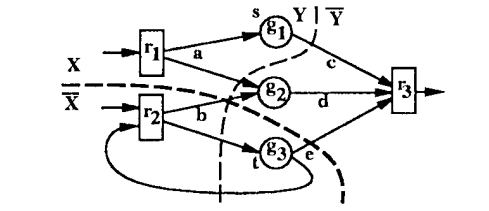
\includegraphics[scale=0.5]{figckt.png}
	\end{center}
	\caption{Circuit nets example}
	\label{fig:ckt}
\end{figure}

Fig.\ref{fig:ckt} is an example netlist with 2 different cut sets. In this figure, net $a$ and $b$
could be represented with hyperedges. Fig.\ref{fig:net} explains a method to translate such nets into
edges that could be dealt with general min-cut algorithm. 2 dummy vertices are inserted as long as a "bridging edge"
with weight 1. Once this net is cut, the bridging edge must be included in the cut set from the output
of any general min-cut algorithm, and cost is 1.

\begin{figure}[hbt]
	\begin{center}
	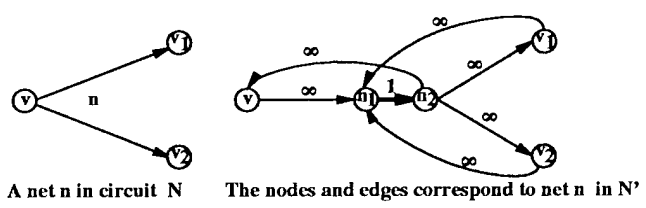
\includegraphics[scale=0.5]{fignet.png}
	\end{center}
	\caption{Transform a Net to subgraph with bridging edge}
	\label{fig:net}
\end{figure}

\begin{algorithm}[hbt]
\caption{Algorithm for constructing flow network from circuit netlists}
\label{alg:construct}
\begin{algorithmic}[1]
\Function{Construct}{Netlist allowing hyperedges $N = (V,E)$}
  \State $V'\gets V$   /*copy all vertices*/
  \For{each net $n\in E$}
  	\State Insert auxiliary vertices $n_1$ and $n_2$ into $V'$
  	\State Insert bridging edge $e = (n_1,n_2)$ with unit weight into $E'$
  	\For{each node $u$ incident to $n$}
  		\State Insert edge $(u,n_1)$ and $(n_2,u)$ with infinite weight into $E'$
  	\EndFor
  \EndFor
  \State \Return graph $N' = (V',E')$
\EndFunction
\end{algorithmic}
\end{algorithm}

It showes from algorithm \ref{alg:construct} that the size of newly constructed graph will not explode.
And the following theorem guarantees that the result of general min-cut algorithm can be adopted.

\begin{Theorem}
$N$ has a cut of net whose size is at most $C$ if and only if $N'$ has a cut of capacity at most $C$.
\end{Theorem}

\subsection{Min-cut Balanced Bipartition}
It is easy to see a minimum cut of nets in netlist can be computed from general min-cut algorithm, based on
our netlist-graph translation. However, the min-cut cannot guarantee a balanced bipartition. It is necessary
to build an algorithm iterating with optimal min-cut and improve the balance every loop, which is the FBB algorithm we want to propose.

\begin{algorithm}
\caption{FBB Algorithm}
\label{alg:FBB}
\begin{algorithmic}[1]
\Function{FBB}{graph $G = (V,E)$}
  \State Randomly pick a pair of vertices as source $s$ and sink $t$, delete all edges starting from $t$ or
  ending at $s$
  \State $C \gets $\Call{MinCut}{$G$}
  \State $X\gets$ vertices from source part $\setminus C$
  \State $X'\gets$ vertices from sink part $\setminus C$
  \While{$C$ violates balancing criteria}
  	\If{$X$ is too small}
  		\State Collapse $X$ to $s$
  		\State Collapse to $s$ a vertex $v\in X'$ adjacent to $C$
  	\Else
  		\State Collapse $X'$ to $t$
  		\State Collapse to $t$ a vertex $v\in X$ adjacent to $C$
  	\EndIf
    \State $C \gets $\Call{MinCut}{$G$}
  \State $X\gets$ vertices from source part $\setminus C$
  \State $X'\gets$ vertices from sink part $\setminus C$
  \EndWhile
  \State \Return $C$
\EndFunction
\end{algorithmic}
\end{algorithm}

\begin{figure*}[hbt]
	\begin{center}
	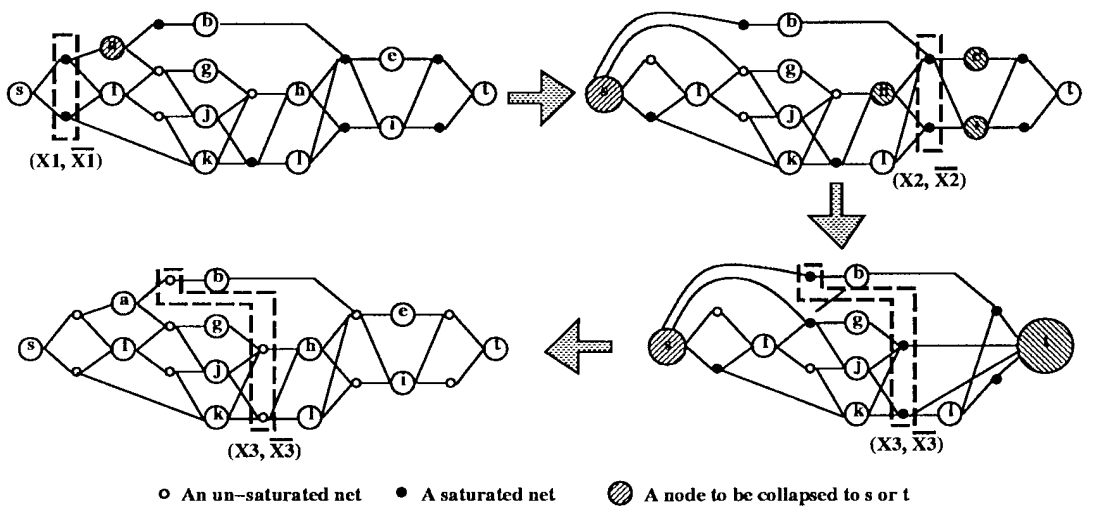
\includegraphics[width=5in]{figfbb.png}
	\end{center}
	\caption{An example on FBB algorithm execution}
	\label{fig:FBB}
\end{figure*}

Fig.\ref{fig:FBB} illustrates what algorithm \ref{alg:FBB} does. First step, $s$ and $t$ are randomly chosen
from all vertices, and a min-cut $(X1,\overline{X1})$ of cost 2 is computed. Note that a small dot denote
a pair of auxiliary nodes we added for each net. Apparently this is not a balanced cut 
partition, so we merge $X$ ($\varnothing$ in first iteration) into $s$, then pick vertex $a$ from $X'$, also
merge it into $s$. In the second iteration, we run min-cut algorithm again, and get a cut $(X2,\overline{X2})$.
The cost is also 2, but this is still not balanced in the other direction. This time we merge $X'$ 
(vertices $e$ and $i$) into $t$, as well as vertex $h$ chosen from $X$. In third iteration, a cut $(X3,\overline{X3})$ of cost 3 satisfies the balancing criteria, which is returned as final result.

\subsection{Efficient Min-cut Computation}
The algorithm's complexity is retarded by computing min-cut within each iteration. In order to improve this,
a new incremental flow computation based algorithm is proposed. The main idea is to keep track of the flow
information from last iteration, and start the max-flow computing from this initial flow instead of zero flow.

\begin{algorithm}
\caption{Incremental Flow Min-cut}
\label{alg:incflow}
\begin{algorithmic}[1]
\Function{IncFlowMinCut}{residue flow graph $G'$}
	\State copy flow info from last iteration
  \While{$\exists$ an augmenting path from $s$ to $t$}
  	\State saturate this path
  \EndWhile
  \Comment/* there is no more augmenting path from $s$ to $t$ */
  \For{all vertices $u$}
  	\If{$\exists$ an augmenting path from $s$ to $u$}
  		\State Insert $u$ to set $X$
  	\EndIf
  \EndFor
  \For{all vertices $u\in X$}
  	\If{$e=(u,v)$ is bridging edge and $v\notin X$}
  		\State Insert $e$ into $C'$
  	\EndIf
  \EndFor
  \State \Return $C$ whose nets contain $C'$ as min-cut
  \State \Return $X$, and $V'\setminus(X\cup C')$ as $X'$
\EndFunction
\end{algorithmic}
\end{algorithm}

The refined algorithm with $k$ iterations is proved to have same complexity as a zero-flow min-cut algorithm.

\section{Experiment}
I plan to execute experiment on ISCAS benchmarks, and do comparison with K-L based tools and \emph{\HMetis} tool.
This heuristic depends on the initial assignment of source and sink, so FBB should be executed for multiple
times to test average performance.



%%%%%%%%%%%%%%%%%%%% The bibliography %%%%%%%%%%%%%%%%%%%%%%%%%%%%
\begin{thebibliography}{1}
\bibitem{ref1}
Yang H H, Wong D F. \emph{Efficient network flow based min-cut balanced partitioning}[M], The Best of ICCAD. Springer US, 2003: 521-534.
\end{thebibliography}
\end{document}


%%%%%%%%%%%%%%%%%%%%%%%%%%%  End of IEEEsample.tex  %%%%%%%%%%%%%%%%%%%%%%%%%%%
